
% !TEX encoding = UTF-8 Unicode
% !program = pdflatex

\documentclass[a4paper,11pt]{article}
\usepackage[a4paper,top=38mm,right=16mm,bottom=24mm,left=25mm,head=35mm,foot=15mm]{geometry}
\usepackage[comma]{natbib}
\bibliographystyle{agsm}
\usepackage[english]{babel}
\usepackage{tocbibind}

% font
\usepackage[utf8]{inputenc}
\usepackage{graphicx}
\graphicspath{ {images/} }
\usepackage[T1]{fontenc}
\usepackage[parfill]{parskip}
\usepackage{soul,rotating}
\usepackage{pdflscape}

\usepackage{helvet}
\renewcommand*\familydefault{\sfdefault}


% syntax highlighting of code
\usepackage{listings}
\usepackage{color}
\definecolor{gray}{rgb}{0.4,0.4,0.4}
\definecolor{darkblue}{rgb}{0.0,0.0,0.6}
\definecolor{cyan}{rgb}{0.0,0.6,0.6}

\lstset{
  basicstyle=\ttfamily,
  columns=fullflexible,
  showstringspaces=false,
  commentstyle=\color{gray}\upshape
}

\lstdefinelanguage{XML}
{
  numbers=left,
  numberstyle=\scriptsize,
  morestring=[b]",
  morestring=[s]{>}{<},
  morecomment=[s]{<?}{?>},
  stringstyle=\color{black},
  identifierstyle=\color{darkblue},
  keywordstyle=\color{cyan},
  frame=lines,
  morekeywords={xmlns,version,type,rdf,fam}
}

\lstdefinelanguage{GraphQL}
{
  numbers=left,
  numberstyle=\scriptsize,
  morestring=[b]",
  morestring=[s]{>}{<},
  morecomment=[s]{<?}{?>},
  stringstyle=\color{black},
  identifierstyle=\color{darkblue},
  keywordstyle=\color{cyan},
  frame=lines,
  morekeywords={xmlns,version,type,rdf,fam}
}

\lstdefinelanguage{JSON}{
    numbers=left,
    numberstyle=\scriptsize,
    stepnumber=1,
    numbersep=1pt,
    showstringspaces=false,
    breaklines=true,
    frame=lines,
    literate=
     *{0}{{{\color{cyan}0}}}{1}
      {1}{{{\color{cyan}1}}}{1}
      {2}{{{\color{cyan}2}}}{1}
      {3}{{{\color{cyan}3}}}{1}
      {4}{{{\color{cyan}4}}}{1}
      {5}{{{\color{cyan}5}}}{1}
      {6}{{{\color{cyan}6}}}{1}
      {7}{{{\color{cyan}7}}}{1}
      {8}{{{\color{cyan}8}}}{1}
      {9}{{{\color{cyan}9}}}{1}
      {:}{{{\color{darkblue}{:}}}}{1}
      {,}{{{\color{darkblue}{,}}}}{1}
      {\{}{{{\color{black}{\{}}}}{1}
      {\}}{{{\color{black}{\}}}}}{1}
      {[}{{{\color{black}{[}}}}{1}
      {]}{{{\color{black}{]}}}}{1}
}

\usepackage{qtree}
% other
\linespread{1.25}

% variable definitions
\providecommand{\documenttitle}{Linked data-driven UI for task-based computing}

% configure title page
\title{
  
\includegraphics[width=20cm]{images/en-zhaw-init-rgb}\\[\bigskipamount]
  \documenttitle\\[\bigskipamount]
}

\author{Josef Erben
  \\[1cm]{\small Main advisor: Philipp Hofmann}
  \\{\small Advisor: Alain Lafon}
  \\{\small Industrial partner: Miko Nieminen Consulting}
}

\date{\parbox{\linewidth}{\centering%
  Date 07.06.2019 \endgraf
}}

% table
\usepackage{array}
\usepackage{multicol}
\usepackage{longtable,tabu,booktabs}

% links
\usepackage{hyperref}
\hypersetup{
            pdftitle={Linked data driven UI for task-based computing},
            pdfauthor={Josef Erben},
            colorlinks=true,
            linkcolor=[RGB]{74,144,226},
            citecolor=[RGB]{74,144,226},
            urlcolor=[RGB]{74,144,226},
            breaklinks=true}
\urlstyle{same} 
\newcommand*{\fullref}[1]{\hyperref[{#1}]{\nameref*{#1} (\ref*{#1})}}

% images
\usepackage[font=small,skip=6pt]{caption}
\usepackage{float,graphicx,grffile,wrapfig}
\graphicspath{ {images/} }

\makeatletter
\def\maxwidth{\ifdim\Gin@nat@width>\linewidth\linewidth\else\Gin@nat@width\fi}
\def\maxheight{\ifdim\Gin@nat@height>\textheight\textheight\else\Gin@nat@height\fi}
\makeatother
\setkeys{Gin}{width=\maxwidth,height=\maxheight,keepaspectratio}

\makeatletter
\def\fps@figure{H}
\makeatother

% header and footer
\usepackage{lastpage}
\usepackage{fancyhdr}
\pagestyle{fancy}
\fancyhf{}
\fancyhead[L]{
\includegraphics[height=1.5cm]{images/zhaw-small}}
\fancyfoot[L]{\fontsize{8}{10}\selectfont\ \documenttitle}
\fancyfoot[R]{\fontsize{8}{10}\selectfont\ Page\ \thepage\ of\ \pageref*{LastPage}}

\renewcommand{\headrulewidth}{0pt}
\renewcommand{\footrulewidth}{0pt}

% glossary
\usepackage[toc]{glossaries}
 
\makeglossaries
\loadglsentries{glossary}

% headers
\usepackage{titlesec}

\begin{document}
\selectlanguage{english}

\maketitle\thispagestyle{empty}\newpage

\begin{abstract}
  Accidental Complexity in contemporary software development is high, especially in UI development. A big chunk of UI development time is not spent on delivering business value but infrastructure work. This thesis explores an efficient approach to UI development by reducing Accidental Complexity.

We analyze hypermedia specifications and develop a proof of concept for a framework to create user interfaces by implementing two use cases. The first use case is a scenario in home automation and it is concerned with non-interactive user interfaces. The second use case describes a project management tool with focus on user interaction.

The combination of linked data, web components and \textit{Hypermedia As The Engine Of Application State} reduces the complexity in development of user interfaces. Usage of the implemented framework reduces \gls{cognitive load}, decreases \textit{Complexity caused by State} and \textit{Complexity caused by Control} and significantly drives down maintenance costs.

The suggested approach to development of user interfaces constitutes an improvement over approaches without linked data and hypermedia.

  \newpage
\end{abstract}

{
  \hypersetup{linkcolor=black}
  \tableofcontents
}

\section{Introduction}\label{introduction}

\begin{quotation}
\textit{``There is no single development, in either technology or management technique, which by itself promises even one order-of-magnitude improvement within a decade in productivity, reliability, in simplicity.''} \citep{nosilverbullet}
\end{quotation}

Frederick P. Brooks, Jr. states this in his work \textit{No Silver Bullet} where he looks for a silver bullet to \textit{lay the werevolves of software complexity to rest} \citep{nosilverbullet}.

He breaks down software complexity and describes that reduction of software complexity is more feasible for some types than others.

This thesis explores the generation of user interfaces (\gls{ui}s) for application programming interfaces (\gls{api}s) that fulfill certain criteria in the context of the World Wide Web. The main goal is to reduce the manual work required in UI development. The goal of this thesis is to decrease costs of UI development by reducing the involved complexity.

\subsection{Context}\label{context}
In order for information systems to be useful, they either have to interact with other systems or with human users. Those systems are increasingly more connected together and they exchange data without any human interaction. When it comes to human-computer interaction, UIs are implemented that consume HTTP APIs which use the JSON data format \citep{jsonformat}. Those UIs are part of mobile, desktop or browser-only applications. End users interact with those applications through UIs in order to carry out tasks.

\subsection{Problem}\label{problem}
The contemporary way of implementing those UIs involves a lot of manual work. JSON is a very popular format for data exchange between information systems in web development. While humans can often infer the meaning of a piece of JSON data, it is not trivial for machines to do so. Specific knowledge about the JSON data is needed for a machine to understand the meaning of it. That specific knowledge is only valid for a certain API in a certain context. It is manually, often implicitly, encoded into the application which contains the UI as shown in figure \ref{fig:hardcoded}. This knowledge is required to understand the data coming from such an API, it gives the data its \textbf{semantics}. These client applications are strongly coupled to specific APIs and can not be re-used. Instead, client applications are written from scratch to work with slightly different APIs which often share the same or similar data models.

Current approaches fail to exploit the architecture of the World Wide Web and they completely ignore the possibilities offered by \textbf{linked data}.

\begin{figure}[!htb]
  \center{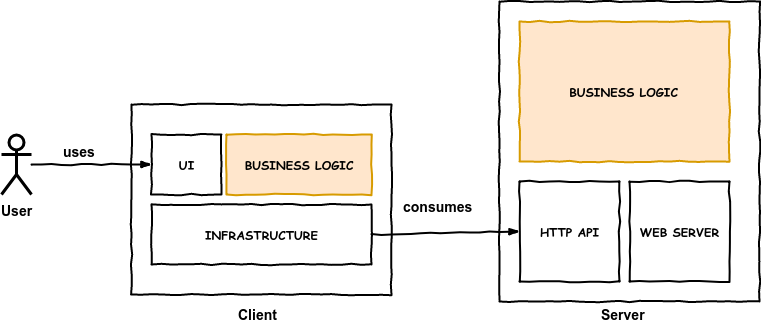
\includegraphics[width=450pt]
    {images/ui-dev-now.png}}
  \caption{A part of the business logic is hard coded into the client.}
  \label{fig:hardcoded}
\end{figure}

\subsection{Strategy}\label{strategy}
With this thesis we aim to identify types of complexity in UI and web development and suggest an approach to reduce them.
We want to minimize the manual work by leveraging linked data, the declarative concept of web components, the interaction model of task-based computing and by using hypermedia.

The expected results and artifacts consist of a proof-of-concept for a UI framework, n HTTP hypermedia vocabulary based on linked data, an interaction model influenced by task-based computing and the implementation of two use cases that showcase the UI framework. \\
Furthermore, we evaluate the UI framework in terms of its effect on software complexity. By reducing the complexity we aim to reduce the overall costs in UI and web development.

\subsection{Industrial partner}
The industrial partner of this thesis is Miko Nieminen Consulting. Miko Nieminen Consulting is interested in pushing open source efforts in linked data driven UI with complex user interaction. A future real-world use case is the generation of UIs for administrators.

\section{Background}\label{background}

This section discusses the problems with the process of developing UIs today. It also provides the theoretical backgroung by highlighting the main building blocks of the UI framework.

\subsection{Accidental and Essential Complexity}\label{history}

According to Turing Award winner Fred Brooks there are two types of complexity: accidental complexity and essential complexity. \citep{nosilverbullet}
In software engineering, \textbf{essential complexity} is complexity that comes from the domain problem that we want to solve. It is inherent to the problem that the customer cares about and its solution delivers business value. \textbf{Accidental complexity} is complexity that is caused by everything else. Compilers, distributed systems and databases are all examples for accidental complexity. In fact even programming languages and computers are often accidental complexity since they are not essential to the customer's problem.

This implies that accidental complexity could be eradicated in an ideal world. An example of such scenario is an executable specification: It comprises only business rules which are essential to the problem of the business, it doesn't contain any accidental complexity.

Ben Moseley and Peter Marks explore a general infrastructure to run specifications in their paper Out of the Tar Pit \citep{outoftarpit}.

Software engineering is itself an everlasting fight against accidental complexity. This is indeed the main goal of the UI Framework.

\subsection{Evolution of UI web development}\label{history}

In the early days of the Internet, websites were mostly \textbf{static files} accessible under certain URLs. Those files were often created manually or generated by using WYSIWYG editors. The served files were mostly styles (CSS), static assets and markup that the browsers had to render.

\textbf{Dynamically generated} content became popular with the rise of PHP. Websites were now able to show different things to each user based on previous interactions. The files that were served to the browsers were still the same static files. The markup was not hard coded anymore but dynamically rendered on the server upon user request.
\\ Developers had to work with templating languages to implement UIs that received that usually from the same server.

Websites became \textbf{truly interactive} with the introduction of AJAX. AJAX allowed the browser to asynchronously communicate with the server while the user was interacting with the website. Google was able to give search suggestions in real-time while the user was typing the search term. Websites were still rendered on the server but the served files additionally contained JavaScript that was run by the browser.
\\ UI development involved working with templating languages, styling and a small amount of programming.

The amount of interactive elements on websites and their \textbf{complexity increased}. What was once a text input field with real-time suggestions is now a full-text search interface with complex filtering and sorting options. The standardization of browser APIs was in the early stages and developers had to spend effort to create a consistent user experience across various browsers.
\\ Tools like jQuery emerged that provided a single interface for multiple browsers. The websites were still dynamically rendered on the server and just enriched in the browser by running JavaScript.

The first applications appeared providing a user experience in the browser similar to the one of fat desktop applications. The files that the server sent to the browser were mostly JavaScript. The browser ran that JavaScript application to render the website and to react on user input. It communicated with the server using AJAX and the website was not rendered on the server anymore. Instead a single website was served on which the whole application lifecycle took place. \textbf{Single page applications} (SPA) were born.
\par Development of UIs has drastically changed because the UI was part of an application that had its own lifecycle. Development of the server and the client application often took place separated. The HTTP API often played the role of an informal contract between client and server.

\subsection{Document Object Model}\label{documentobjectmodel}

The Document Object Model (DOM) is a programming API for HTML and XML documents. It defines the logical structure of documents and the way a document is accessed and manipulated. \citep{dom} The DOM exposes an \textbf{imperative} API to the developer.

We consider following HTML document:

\lstset{language=XML}
\begin{lstlisting}[caption=HTML document of a table, label=htmloftable]
<table>
  <rows>
    <tr>
      <td>Walter</td>
      <td>White</td>
    </tr>
    <tr>
      <td>Saul</td>
      <td>Goodman</td>
    </tr>
  </rows>
</table>
\end{lstlisting}

The DOM representation of that table looks as follows:

\begin{figure}[!htb]
  \center{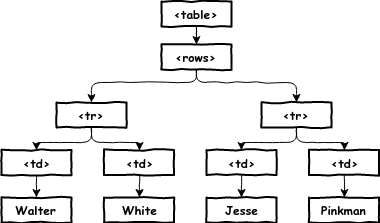
\includegraphics[width=250]
    {images/dom.png}}
  \caption{\label{fig:my-label} The DOM is a tree data structure representing an HTML document.}
\end{figure}

This process of creating the DOM given a document with markup takes place in the browser during \textbf{rendering}.

\subsection{UI web development today}\label{uidevelopmenttoday}

To this day a lot of UIs are developed that way. Some parts are increasingly rendered on the server again, mainly for performance and search engine optimization. It is common to have a \textbf{frontend} team working on the client and a \textbf{backend} team working on the server. The frontend team makes sense of the data that comes from the server either manually or in the best case using some form of HTTP API documentation.
\\ There are efforts like Swagger or OpenAPI to formalize and standardize documentation of HTTP APIs. Often documentation can be generated to a certain extent, so the overhead to keep the up-to-date is small. Documentation helps \textbf{humans} (frontend team) to understand the data and to develop a client that consumes the documented API in an efficient and effective way.
\\ Nevertheless, data coming from the server has to be understood by human frontend developers. That interpretation of the meaning of the incoming data is hard coded into the client and the UI. This causes strong coupling of the client to the data and therefore to the server. The client can not be re-used in some other \textbf{context}.

\subsubsection{Lack of context}\label{datahumanmachine}

Picture a scenario in everyday life where two good friends meet. One of them says: \textit{Have you heard about Frank? He recently got married.} Chances are high the other one knows multiple people named \textbf{Frank}. Being a human, he is able to map the name \textbf{Frank} to the person the other one is referring to. He is able to do so, because that conversation has an implicit context. That context is the intersection of the sets of people \textbf{both know}.
\par Exactly the same thing happens frequently in software development, especially in data exchange. A frontend developer looks at either all HTTP routes of an API or glances over the documentation. Sometimes he is able to \textbf{infer} the domain model because of his personal experiences as a human. If that developer is not familiar with the domain at all, maybe because the domain is niche, he has trouble understanding the data coming from the server. He perceives development to be difficult and he is not able to put the data being exchanged into a \textbf{context}.
\par What makes the life of a human developer hard, poses an insurmountable obstacle to a machine. A machine doesn't have dozens of years of life experience to draw from when trying to understand data.\footnote{Here we talk about machines in the sense of contemporary information systems. Systems that are able to learn are deliberately ignored as they haven't been proven to be useful in this context.} The machine has to be fed a context together with the data it should understand. In traditional web UI development that context is hard coded into the client and the UI. The author believes that the majority of work done in UI development could be eliminated by \textbf{exchanging data that has meaning attached to it}.

\subsection{Web components}\label{webcomponents}

In recent years an approach to rendering UIs became popular which we will call \textbf{component-based} rendering. This paragraph analyzes the reason why this approach to UI development gained popularity.

\subsubsection{React}

In 2013 Facebook released a library called React, which today is still one of the main tools for web development. It was one of the first libraries to encourage the usage of \textbf{web components}. Due to its widespread adoption in web development it caused a paradigm shift.

React encourages the thinking of UIs as a composition of \textbf{web components}. The UI developer doesn't touch the DOM manually and merely provides data to React. This is a declarative approach where the developer states \textbf{what} not \textbf{how} the UI should be rendered. \\
Most importantly, React models the problem of UI rendering as function application. This insight leads to small re-usable components which has various benefits.


\begin{figure}[!htb]
  \center{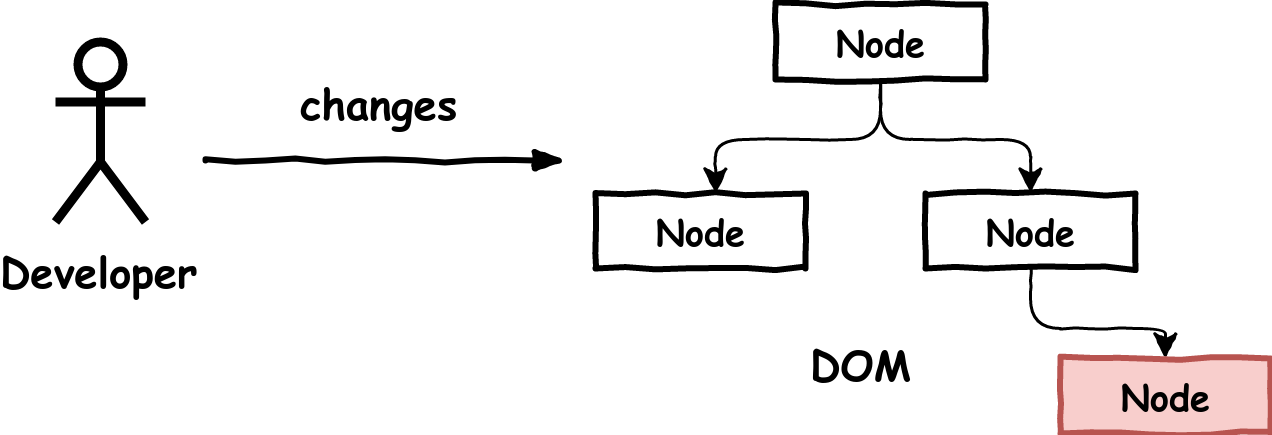
\includegraphics[width=250]
    {images/ui-imperative.png}}
  \caption{\label{fig:my-label} Imperative development: Developer works directly with DOM.}
\end{figure}

\begin{figure}[!htb]
  \center{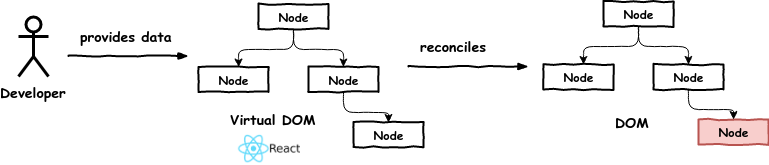
\includegraphics[width=380]
    {images/ui-declarative.png}}
  \caption{\label{fig:my-label} Declarative development: Developer provides data and React takes care of the DOM.}
\end{figure}

The markup output of a component depends only on its data input. This allows to understand the change in the output when changing the input, the component is \textbf{easy to reason about}. It can be \textbf{tested easily in isolation} because there are no other dependencies than the data input. Analogous to function composition, such web components can be \textbf{composed} to larger UIs. Because web components are designed to be self-contained, they have high cohesion which makes them usable in multiple contexts. That means a good code \textbf{reuse can be achieved}.

\subsubsection{Templates vs. Component}

TODO: Quote Riotjs

\subsection{Richardson Maturity Model and HATEOAS}

TODO

\subsection{Linked data}\label{linkeddata}

Linked data is a way of creating a web of machine interpretable data across different domains, systems and organizations. A person or a machine should be able to explore data by simply following links. In essence, the same expectations apply to make that web of data grow as to linked HTML documents: \citep{linkedatafourrules}

\begin{enumerate}
  \item Use URIs as names for things
  \item Use HTTP URIs so that people can look up those names.
  \item When someone looks up a URI, provide useful information, using the standards (RDF*, SPARQL)
  \item Include links to other URIs, so that they can discover more things.
\end{enumerate}

A machine looking at a piece of linked data follows the links and is able to unambiguously understand the data. This is equivalent of traversing a graph since linked data is effectively a giant graph. There are multiple serialization formats in the family of specifications called Resource Description Framework (RDF) \citep{rdfspecification}.

An RDF file describing a Smith family could live at \lstinline{http://example.org/smith} and have following content:

\lstset{language=XML}
\begin{lstlisting}[caption= Simple example of a person as RDF, label=rdfexample]
<rdf:Description about="#albert"
 <fam:child rdf:Resource="#brian">
  <fam:child rdf:Resource="#carol">
  </rdf:Description>
\end{lstlisting}

Information about the grandparent Albert can be obtained by loading the data at \\ \lstinline{http://example.org/smith#albert}. Albert's child Brian can be accessed at \\  \lstinline{http://example.org/smith#brian} and Brian's child Carol at \lstinline{http://example.org/smith#carol}.

\subsection{JSON-LD}\label{jsonld}

TODO mention users of JSON-LD: https://github.com/json-ld/json-ld.org/wiki/Users-of-JSON-LD

In web development the main format for data exchange now is JSON \citep{jsonformat}. It is easy to parse and to generate and many languages provide first-class support for it.

However, JSON is difficult to integrate from different sources as the data may contain keys that conflict with other data sources. JSON has no built-in support for hyperlinks, which are a fundamental building block on the Web \citep{jsonldbasicconcepts}.

Consider following JSON snippet:

\lstset{language=JSON}
\begin{lstlisting}[caption=Data of a person in the JSON format, label=jsonexample]
{
  "name": "Manu Sporny",
  "homepage": "http://manu.sporny.org/",
  "image": "http://manu.sporny.org/images/manu.png"
}
\end{lstlisting}

It's obvious to humans that the data is about a person whose name is \textit{Manu Sporny} and that the homepage property contains the URL of that person's homepage. A machine doesn't have such an intuitive understanding and sometimes, even for humans, it is difficult to resolve ambiguities in such representations. This problem can be solved by using unambiguous identifiers to denote the different concepts instead of tokens such as \textbf{name} or \textbf{homepage} \citep{jsonldbasicconcepts}.

JSON-LD is a serialization format for linked data and is based on JSON-LD. By using the popular schema.org vocabulary the example \ref{jsonexample} can be written as follows:

\lstset{language=JSON}
\begin{lstlisting}[caption=Data of a person in the JSON-LD format, label=jsonldexample]
{
  "http://schema.org/name": "Manu Sporny",
  "http://schema.org/url": {
    "@id": "http://manu.sporny.org/"
  },
  "http://schema.org/image": {
    "@id": "http://manu.sporny.org/images/manu.png"
  }
}
\end{lstlisting}

This can be understood by any machine without providing additional information. The key \lstinline{http://schema.org/name} can be looked up to determine the meaning of the value \lstinline{Manu Sporny}. JSON-LD supports the concept of a \textbf{context}.

The context is meta data that has to be provided together with the data. This makes it possible for a machine to attach meaning to it. Thanks to the context it is not required to have the keys as absolute URIs anymore. The data can be compacted and written as follows:

\lstset{language=JSON}
\begin{lstlisting}[caption=Compacted data of a person, label=jsonldcompacted]
{
  "@context": "http://schema.org",
  "name": "Manu Sporny",
  "url": "http://manu.sporny.org/",
  "image": "http://manu.sporny.org/images/manu.png"
}
\end{lstlisting}

With the small addition of the reserved keyword \lstinline{@context} readability of JSON was restored while allowing machines to understand the data. JSON-LD is 100\% compatible with JSON and therefore benefits of the vast amount of JSON tooling available.

There are a few operations that can be executed on JSON-LD. Following are the three most important ones for this thesis:

\subsubsection{Framing}\label{jsonldframing}

Framing is an operation that re-shapes the data. Input of the framing operation is data and a \textbf{frame}. The frame determines the new shape of the data.

Consider following data of a library. The data is in the form of a normalized graph. The \lstinline{contains} relation represents edges between nodes, the items in the \lstinline{@graph} list are the graph nodes.

\lstset{language=JSON}
\begin{lstlisting}[caption=Data of a library as normalized graph]
{
  "@context": {
    "@vocab": "http://example.org/",
    "contains": {"@type": "@id"}
  },
  "@graph": [{
    "@id": "http://example.org/library",
    "@type": "Library",
    "contains": "http://example.org/library/the-republic"
  }, {
    "@id": "http://example.org/library/the-republic",
    "@type": "Book",
    "creator": "Plato",
    "title": "The Republic",
    "contains": "http://example.org/library/the-republic#introduction"
  }, {
    "@id": "http://example.org/library/the-republic#introduction",
    "@type": "Chapter",
    "description": "An introductory chapter on The Republic.",
    "title": "The Introduction"
  }]
}
\end{lstlisting}

Following frame determines the shape of the frame data:

\lstset{language=JSON}
\begin{lstlisting}[caption=Frame for the framing operation]
{
  "@context": {
    "@version": 1.1,
    "@vocab": "http://example.org/"
  },
  "@type": "Library",
  "contains": {
    "@type": "Book",
    "contains": {
      "@type": "Chapter"
    }
  }
}
\end{lstlisting}

The result of the framing operation is a tree:

\lstset{language=JSON}
\begin{lstlisting}[caption=Framed data of a library]
{
  "@context": {
    "@version": 1.1,
    "@vocab": "http://example.org/"
  },
  "@id": "http://example.org/library",
  "@type": "Library",
  "contains": {
    "@id": "http://example.org/library/the-republic",
    "@type": "Book",
    "contains": {
      "@id": "http://example.org/library/the-republic#introduction",
      "@type": "Chapter",
      "description": "An introductory chapter on The Republic.",
      "title": "The Introduction"
    },
    "creator": "Plato",
    "title": "The Republic"
  }
}
\end{lstlisting}

\subsubsection{Compacting}\label{jsonldcompacting}

Compacting describes the operation of reducing verbosity in the JSON-LD data. Compacted data is meant to be read and understood by human developers. This is achieved by pulling out the context and explicitely define it using the \lstinline{@context} keyword.

Consider following input:

\lstset{language=JSON}
\begin{lstlisting}[caption=Verbose data of a person]
{
  "http://schema.org/name": "Manu Sporny",
  "http://schema.org/url": {
    "@id": "http://manu.sporny.org/"
  },
  "http://schema.org/image": {
    "@id": "http://manu.sporny.org/images/manu.png"
  }
}
\end{lstlisting}

This data can be compacted by pulling out the \lstinline{@context}:

\lstset{language=JSON}
\begin{lstlisting}[caption=Compacted and easy-to-read data of a person]
{
  "@context": "http://schema.org",
  "name": "Manu Sporny",
  "url": "http://manu.sporny.org/",
  "image": "http://manu.sporny.org/images/manu.png"
}
\end{lstlisting}

\subsubsection{Expanding}\label{jsonldextending}

Expanded data serves the opposite goal of compacting data. While compacted data is easy to read for humans, extended data is easy to process for machines.

Expanding the following compacted data

\lstset{language=JSON}
\begin{lstlisting}[caption=Compacted and easy-to-read data of a person]
{
  "@context": "http://schema.org",
  "name": "Manu Sporny",
  "url": "http://manu.sporny.org/",
  "image": "http://manu.sporny.org/images/manu.png"
}
\end{lstlisting}

results in following expanded data:

\lstset{language=JSON}
\begin{lstlisting}[caption=Expanded data of a person that is easy to process for machines]
[
  {
    "http://schema.org/image": [
      {
        "@id": "http://manu.sporny.org/images/manu.png"
      }
    ],
    "http://schema.org/name": [
      {
        "@value": "Manu Sporny"
      }
    ],
    "http://schema.org/url": [
      {
        "@id": "http://manu.sporny.org/"
      }
    ]
  }
]
\end{lstlisting}

\subsection{Vocabulary}

JSON-LD is essentially a linked data serialization format that plays well with JSON tooling. Creating linked data means creating a vocabulary that other might use by linking to it. A lot of vocabularies those exist and two of them are particularly interesting for this thesis.

\subsubsection{Schema.org}

\url{Schema.org} is a collaborative, community activity with a mission to create, maintain, and promote schemas for structured data on the Internet, on web pages, in email messages, and beyond \citep{welcomeschemaorg}. Companies like Google, Microsoft, Pinterest and Yandex are using it in their tools and products.

Their main goal is to provide a shared vocabulary that web developers can refer to. It is often used in the context of search engine optimization by helping crawlers understand websites.

Schema.org is a hierarchy of \lstinline{Things} that have an implicit \textbf{is a} relationship. This is similar to sub typing through inheritance in many object-oriented programming languages. Following is a small subset of the Schema.org hierarchy:

\begin{figure}[!htb]
  \center{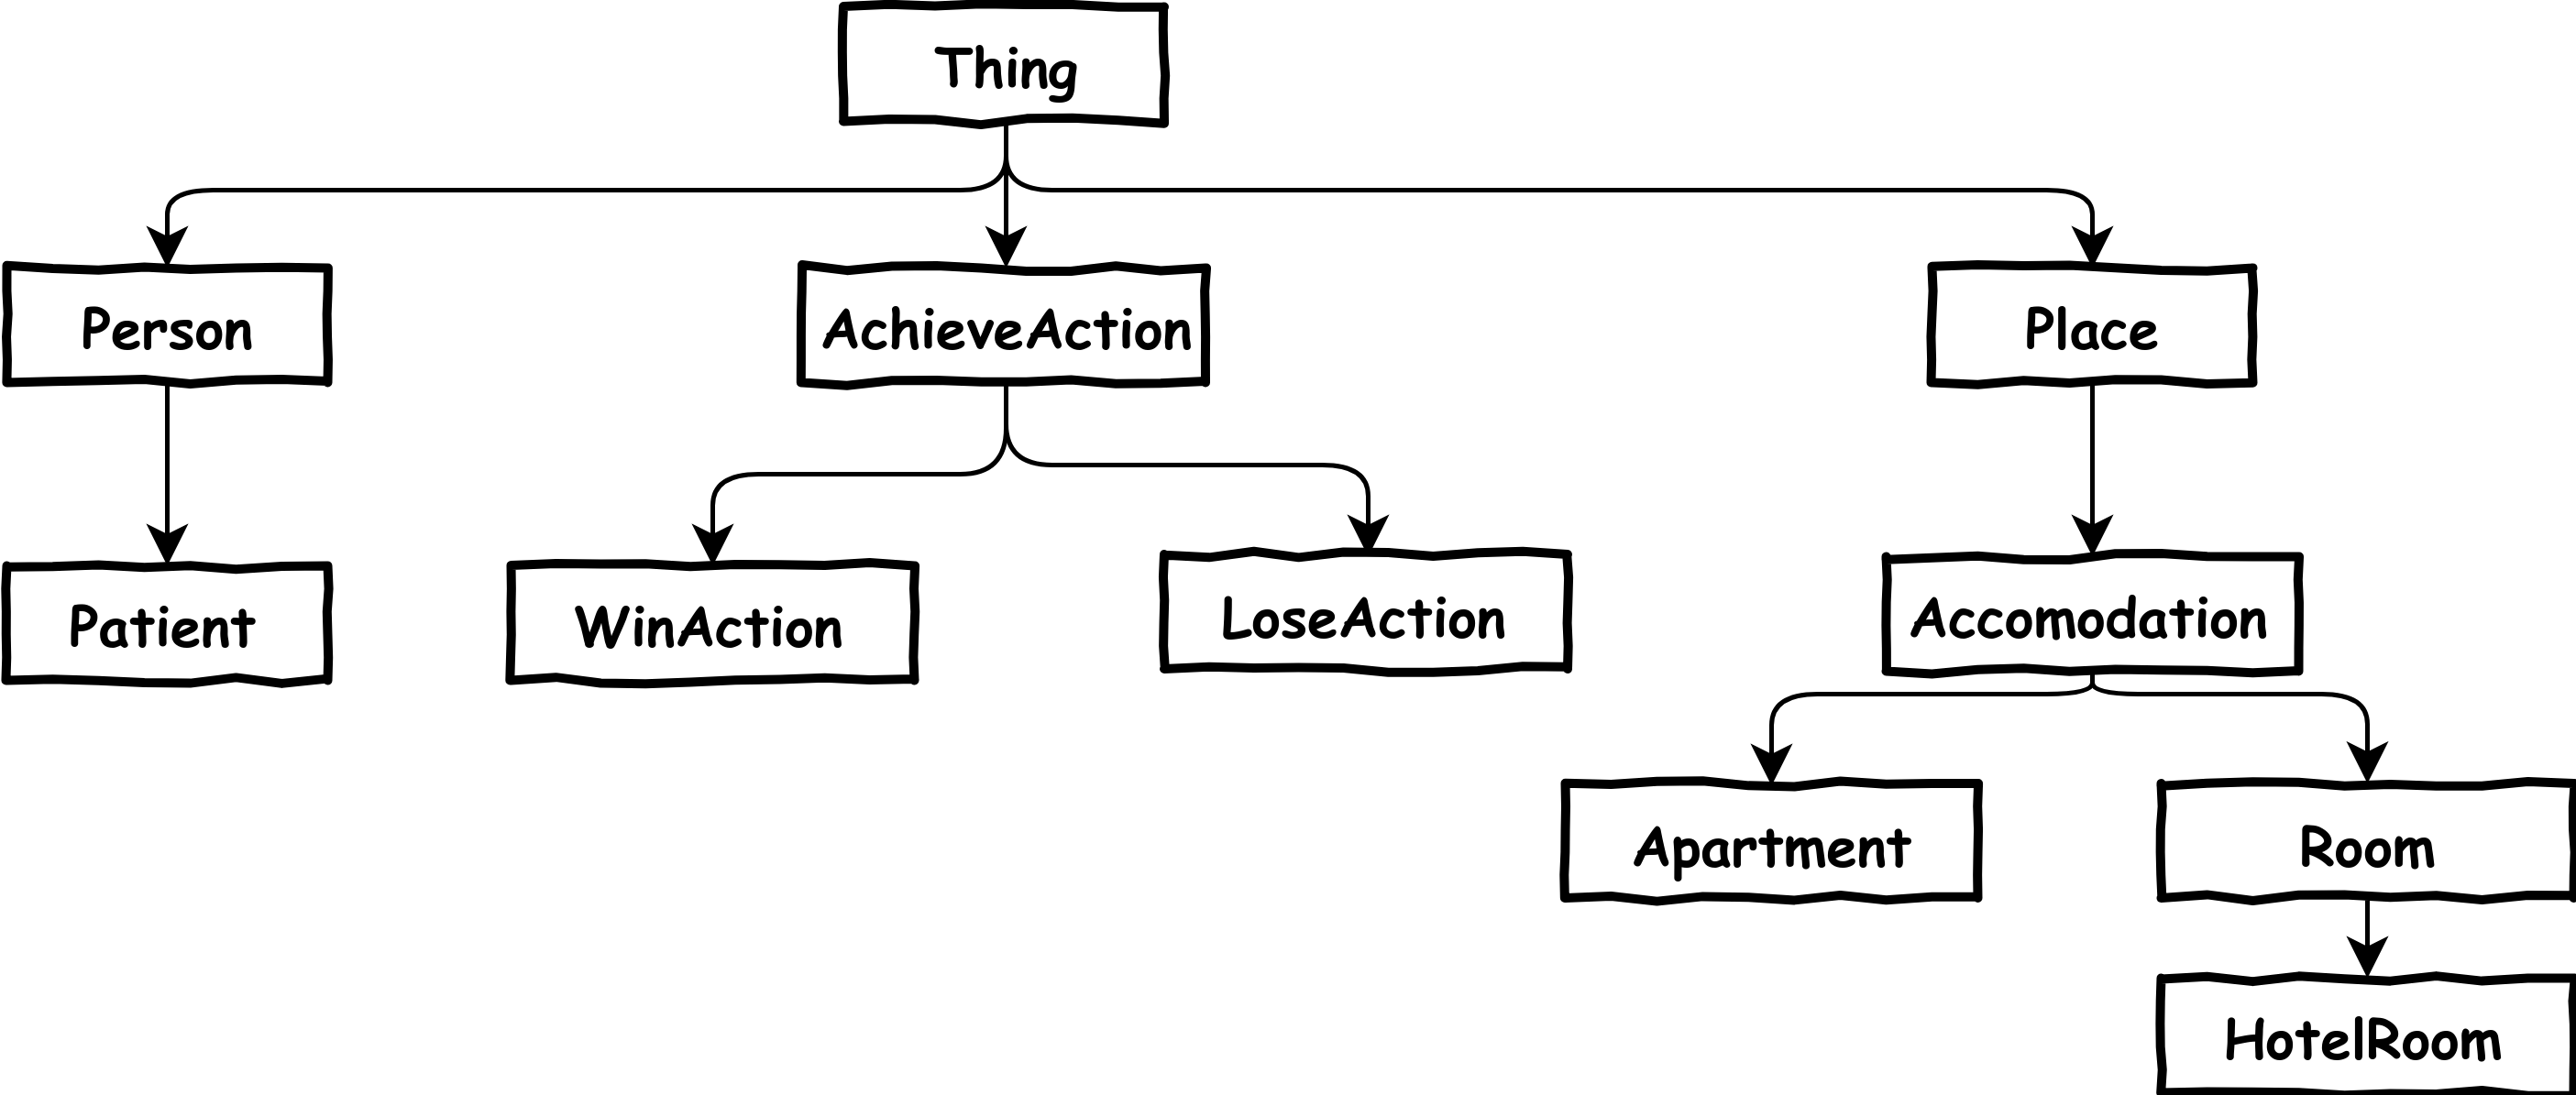
\includegraphics[width=300]
    {images/schemaorg.png}}
  \caption{\label{fig:schemaorg} Subset of the Schema.org ontology where child-parent relation describes an \textit{is a} relationship.}
\end{figure}

The advantage of using such a vocabulary becomes obvious when looking at an example.The type \lstinline{Person} has a property \lstinline{address}. \lstinline{Address} can be of type \lstinline{http://schema.org/Text} or \lstinline{http://schema.org/PostalAddress}.

\lstset{language=JSON}
\begin{lstlisting}[caption=A person with an address of type Text]
{
  "@context": "http://schema.org",
  "givenName": "Walter",
  "familyName": "White",
  "address": "3828 Piermont Dr NE Albuquerque, NM 87111, USA"
}
\end{lstlisting}

A machine receiving that data knows that this is a person and understands his name, but it can not understand his address. There is additional context needed that describes the schema used in the \lstinline{address} property.

The data of the same person where the address is of type \lstinline{http://schema.org/PostalAddress} can be processed unambiguously by any machine that understands linked data.

\lstset{language=JSON}
\begin{lstlisting}[caption=A person with an address of type PostalAddress]
{
  "@context": "http://schema.org",
  "givenName": "Walter",
  "familyName": "White",
  "address": {
    "@type": "PostalAddress",
    "addressLocality": "Albuquerque",
    "addressRegion": "NM",
    "postalCode": "87111",
    "streetAddress": "3828 Piermont Dr NE Albuquerque"
  },
}
\end{lstlisting}

The \lstinline{streetAddress} is still stringly typed. A system running at a package distribution center could route packages correctly to some local distribution center or postal office by looking at \lstinline{addressRegion} and \lstinline{addressLocality}.

\subsubsection{Hydra}

\href{http://www.hydra-cg.com/}{Hydra} is a lightweight vocabulary to create hypermedia-driven Web APIs. By specifying a number of concepts commonly used in Web APIs it enables the creation of generic API clients.\citep{hydasprecs}

\subsection{Landscape of solutions and tools}

\subsubsection{GraphQL}
\subsubsection{Rails with ActiveAdmin}
\subsubsection{Hyperfiddle}
\subsubsection{Fulcro}

\section{Main contributions}\label{contributions}

Lorem ipsum dolor sit amet, consectetur adipiscing elit. Ut ut congue nisl. Maecenas nec odio eget felis ultricies consequat. Vestibulum consequat orci eu augue sodales rhoncus. Sed tempor maximus nisl, in varius eros mollis tempus. Praesent condimentum nibh eros. Maecenas pulvinar massa ut lectus volutpat, ac mattis ligula laoreet. Duis cursus odio a quam ullamcorper, lacinia dignissim magna lobortis. Phasellus nec lectus sit amet elit convallis interdum. Ut at est risus.

Curabitur finibus laoreet mauris at molestie. Nunc arcu est, vulputate sit amet tempus vitae, sagittis in elit. Vestibulum ac pretium justo, vehicula vestibulum lacus. Pellentesque varius mattis aliquet. Vestibulum a lacus placerat, faucibus neque sed, hendrerit ante. Etiam id suscipit odio. Vivamus porta sollicitudin metus, in pulvinar lorem maximus et. Pellentesque eget sodales lacus, et convallis augue. Fusce porta leo et posuere cursus.

\section{Evaluation}
In the following paragraph we evaluate the proof of concept for the UI framework. We examine whether the design goals have been met and we analyze the change in complexity.

\subsection{Design goals}
By looking at the implementations of both use cases, we evaluate whether the design goals defined in \ref{sec:designgoals} have been met.

\subsubsection{Play nicely with others}
Playing nicely with other technologies, existing consumers and existing tooling is the major design goal as described in section \ref{sec:playnice}. Choices on the technologies being used in the UI framework have the biggest impact on it.

\paragraph{JSON-LD}
JSON-LD is valid JSON which means that any tool that accepts JSON also accepts JSON-LD.

\paragraph{Hydra operations}
Hydra operations include an  HTTP verb which the client reads to invoke the operation. Given the developer respects the conventions about safe and idempotent HTTP verbs, their invocations are equal to regular HTTP requests. HTTP proxies and caches treat Hydra requests the same as other HTTP requests.

\paragraph{React}
As discussed in section \ref{sec:react}, React is one of the widely used tools for UI development. The proof of concept for the UI framework accepts only custom renderers using React components. Idiomatic React development uses JSX (JavaScript XML) which requires dedicated support in the development environment. \\
HTML templates \citep{htmltemplates}, which are part of the Web component specification, might become a better choice for the DOM rendering component once the tooling has developed.

\paragraph{Summary}
Due to choice of technology this design goal has been fulfilled and we assess it with a \textbf{score of 3}.

\subsubsection{Straightforward upgrade path}
We explore a scenario with a running RESTful HTTP API returning JSON and a client consuming it. The client renders the UI with a custom rendering solution that creates the DOM based on input data. They are generating HTTP API documentation with a custom tool and the documentation is served using another server. The development team evaluates the upgrade path to a Hydra conform API using the UI framework. We discuss the upgrade steps to evaluate if the upgrade path is straightforward or if there is a lot of friction.

\paragraph{Entity serialization}
Serialization of entities to resources remains the same. Adding a header that transmits the context, similar to the \lstinline{@context} property, suffices. The response payload remains the same and existing consumers don't break.

\paragraph{Hydra documentation}
Documentation is served using the meta data mechanism of Hydra. This is again just a response header that points to the documentation of the response resource. The existing API documentation is marked as deprecated. Developers use the Hydra documentation instead of the old one, so that the previous solution can be removed after a grace period.

\paragraph{Hydra operations}
As the current API follows RESTful principles, the concepts of resources and HTTP methods exist. Resources and HTTP methods are directly mapped to Hydra resources and inline operations using the same HTTP method. This change requires careful design as it might break existing consumers. Migrating existing HTTP methods to Hydra in a non-breaking way might lead to a non-idiomatic use of Hydra operations. This approach could serve as a stepping stone towards using all the power that Hydra operations offer.

\paragraph{Summary}
Due to choice of HATEOAS specification and linked data format, it is almost straightforward to upgrade existing RESTful APIs returning JSON. The \textbf{score is 2.5}.

\subsubsection{Customizability}
In order to assess the customizability of the UI framework, we compare the set of UIs that can be implemented using the UI framework with the set of UIs that can be implemented using tools like React.

\paragraph{Plugin mechanism}
The plugin mechanism allows UI developers to map components to data types. It is possible to register a renderer using the wildcard \lstinline{*} type. This activates the renderer on every type. The UI developer can take control over rendering by using wildcards to render a React component with all the response data as input. The set of UIs that can be implemented using the UI framework is equal to the set of UIs that can be implemented using React.

\paragraph{Summary}
This design goal is fulfilled which leads to a \textbf{score of 3}.

\subsubsection{Developer ergonomics}
We analyze the usage of the UI framework by a developer.

\paragraph{Component API}
Every React component that is invoked by the rendering infrastructure gets a Hydra resource and a \lstinline{renderer} JavaScript function as input.

\lstset{language=JSON}
\begin{lstlisting}[caption={React component API for the apartment renderer as shown in figure \ref{fig:apartmentrenderer}.}\label{lst:componentapi}]
  const Apartment = ({resource, renderer}) => {
    const { "https://schema.org/containsPlace": rooms } = resource;
    return (
      <div style={{ position: "relative" }}>
        ...
        {rooms.map((r: any) => {
          return (
            <PositionedRoom
              renderer={renderer}
              data={r}
              key={r["@id"]}
              xPos={xPos}
              yPos={yPos}
            />
            );
        })}
      </div>
    )
  }
\end{lstlisting}

Listing \ref{lst:componentapi} shows the apartment renderer of the home automation use case. The \lstinline{resource} contains the data of the Hydra resource of \lstinline{@type} \lstinline{https://schema.org/Apartment}. It accesses the property \lstinline{https://schema.org/containsPlace} to fetch the rooms of the apartment. The \lstinline{renderer} function can be invoked with a Hydra resource. This returns the control of the rendering process to the rendering infrastructure.

This allows UI developers to think in terms of data types and self-contained components. Developing isolated components without thinking about mapping data to children components reduces \gls{cognitive load}.

\paragraph{Learning curve}
The learning curve of the UI framework is the sum of the learning curves of JSON-LD, React and Hydra. The knowledge required to create and register custom renderers is trivial and can be neglected in this discussion. \\
Superficial knowledge about JSON-LD is sufficient to use the UI framework. If the developer is only concerned with rendering non-interactive UIs, knowledge about the two the two special JSON-LD properties like \lstinline{@type} and \lstinline{@id} is enough. \\
Although Alcaeus hides implementation details of Hydra, UI developers should know about operations, classes, documentation and collections in order to create interactive UIs. Deep understanding of Hydra and the Hydra client Alcaeus are required for debugging. \\
The learning curve of using React with the UI framework is flat compared to using React standalone. The developer doesn't have to care about topics like state management and client side routing. React has a mature ecosystem covering these things that comes with a certain cognitive overhead. Using the UI framework, developers can focus on learning React without the usual tooling.

\paragraph{Summary}
The learning curve to implement non-interactive UIs is minimal. The component API and renderer registering are simple - the developer can focus on non-infrastructure topics. Implementation of interactive UIs requires good understanding of Hydra. We assess the score of developer ergonomics \textbf{to be 2}.

\subsubsection{Summary}
We rate the design goal \textbf{play nicely with other} with 3, \textbf{straightforward upgrade path} with 2.5, \textbf{customizability} with 3 and \textbf{developer ergonomics} with 2 out of 3. \\ The design goals have been completely met with the exception of a straightforward upgrade path. The migration of RESTful HTTP methods to Hydra operations is not straightforward.

\subsection{Reduction of complexity in software development}
This section analyzes whether and how development with the UI framework affects various types of software complexity. This requires a comparison of a traditional non-linked data driven approach to the development workflow using the UI framework.

\paragraph{Baseline scenario} We describe a baseline scenario where a development team is working on a RESTful HTTP API that returns JSON and on a frontend using React. They use Swagger to generate and serve API documentation.

We assess various types of software complexities in order to gauge the change in complexity between the baseline scenario and the same scenario using the UI framework and Hydra. We assume that a change in software complexity is a similar change in software development cost.

\subsubsection{Essential Complexity}
Brooks gives \textbf{Complexity}, \textbf{Conformity}, \textbf{Changeability} and \textbf{Invisibility} as the four properties of software causing Essential Complexity \citep{nosilverbullet}.

\paragraph{Complexity caused by Invisibility}
\textit{``Software is invisible and unvisualizable. Geometric abstractions are powerful tools. The floor plan of a building helps both architect and client evaluate spaces, traffic flows, views. Contradictions and omissions become obvious. Scale drawings of mechanical parts and stick-figure models of molecules, although abstractions, serve the same purpose. A geometric reality is captured in a geometric abstraction. \\ The reality of software is not inherently embedded in space. Hence, it has no ready geometric representation in the way that land has maps, silicon chips have diagrams, computers have connectivity schematics. As soon as we attempt to diagram software structure, we find it to constitute not one, but several, general directed graphs superimposed one upon another. The several graphs may represent the flow of control, the flow of data, patterns of dependency, time sequence, name-space relationships. These graphs are usually not even planar, much less hierarchical. Indeed, one of the ways of establishing conceptual control over such structure is to enforce link cutting until one or more of the graphs becomes hierarchical.''} \citep[p.~4]{nosilverbullet}

The development team starting out with the Hydra API and the UI framework is able to render a fully functional UI without spending any development effort. JSON-LD is rendered as a tree and relationships between resources are apparent. The Hydra renderer displays collections of data as tables. In the baseline scenario, the developers have to spend a considerable amount of effort on infrastructure before they can render tables. The UI framework \textbf{increases visibility slightly} by providing these visualizations out of the box.

We asses the improvement in complexity caused by Invisibility with a \textbf{score of 1}.

\paragraph{Complexity caused by Conformity}
\textit{''Software people are not alone in facing complexity. Physics deals with terribly complex objects even at the "fundamental" particle level. The physicist labors on, however, in a firm faith that there are unifying principles to be found, whether in quarks or in unifiedfield theories. Einstein argued that there must be simplified explanations of nature, because God is not capricious or arbitrary. \\ No such faith comforts the software engineer. Much of the complexity that he must master is arbitrary complexity, forced without rhyme or reason by the many human institutions and systems to which his interfaces must conform. These differ from interface to interface, and from time to time, not because of necessity but only because they were designed by different people, rather than by God. \\ In many cases, the software must conform because it is the most recent arrival on the scene. In others, it must conform because it is perceived as the most conformable. But in all cases, much complexity comes from conformation to other interfaces; this complexity cannot be simplified out by any redesign of the software alone.''} \citep[p.~3]{nosilverbullet}

The UI framework doesn't affect the complexity that emerges from this property.

The \textbf{score is 0}.

\paragraph{Complexity caused by Changeability}
\textit{``The software entity is constantly subject to pressures for change. Of course, so are buildings, cars, computers. But manufactured things are infrequently changed after manufacture; they are superseded by later models, or essential changes are incorporated into later-serial-number copies of the same basic design. Call-backs of automobiles are really quite infrequent; field changes of computers somewhat less so. Both are much less frequent than modifications to fielded software. \\ In part, this is so because the software of a system embodies its function, and the function is the part that most feels the pressures of change. In part it is because software can be changed more easily - it is pure thought-stuff, infinitely malleable. Buildings do in fact get changed, but the high costs of change, understood by all, serve to dampen the whims of the changers.''} \citep[p.~4]{nosilverbullet}

The UI framework decouples the client from the HTTP implementation. The renderers are valid in a broader context because they consume linked data. The UI remains functional as long as the HTTP API conforms to the Hydra specification. By design, it is possible to change the HTTP API while a user is interacting with the UI - without breaking the UI.

The cost of change in the client and the UI is \textbf{drastically} reduced. \textbf{The score of the improvement is 3}.

\paragraph{Complexity caused by Complexity}
\textit{``The complexity of software is an essential property, not an accidental one. Hence, descriptions of a software entity that abstract away its complexity often abstract away its essence. For three centuries, mathematics and the physical sciences made great strides by constructing simplified models of complex phenomena, deriving properties from the models, and verifying those properties by experiment. This paradigm worked because the complexities ignored in the models were not the essential properties of the phenomena. It does not work when the complexities are the essence.''} \citep[p.~3]{nosilverbullet}

The gist of this property is that complexity breeds complexity. If a software system becomes complex, it becomes harder to add new components without code duplication. Due to the existing complexity it might be very hard to understand the code. \\ Decreasing the complexity by reducing the impact of the other three properties improves this point by definition.

This software property is not orthogonal to the other three. It is not possible to gauge the effect on complexity caused by complexity using the UI framework.

\paragraph{Summary}
While it is not possible to get rid of these properties, the UI framework reduces their impact on complexity in the development process. The data that is driving the client and the UI \textbf{is visualized by default} and the \textbf{complexity of changing} the client is massively decreased.

\subsubsection{Accidental Complexity}
\textbf{Out of the Tar Pit} identifies \textbf{Complexity of State} and \textbf{Complexity of Control} as concrete types of Accidental Complexity by building on top of the work of Brooks.

\paragraph{Complexity caused by State}
\textit{``The severity of the impact of state on testing noted by Brooks is hard to over-emphasise. State affects all types of testing — from system-level testing (where the tester will be at the mercy of the same problems as the hapless user just mentioned) through to component-level or unit testing. The key problem is that a test (of any kind) on a system or component that is in one particular state tells you nothing at all about the behaviour of that system or component when it happens to be in another state. \\ The common approach to testing a stateful system (either at the component or system levels) is to start it up such that it is in some kind of “clean” or “initial” (albeit mostly hidden) state, perform the desired tests using the test inputs and then rely upon the (often in the case of bugs ill-founded) assumption that the system would perform the same way — regardless of its hidden internal state — every time the test is run with those inputs.''} \citep[p.~6]{outoftarpit}

\textit{``In addition to causing problems for understanding a system from the outside, state also hinders the developer who must attempt to reason (most commonly on an informal basis) about the expected behaviour of the system “from the inside”. \\ The mental processes which are used to do this informal reasoning often revolve around a case-by-case mental simulation of behaviour: “if this variable is in this state, then this will happen — which is correct — otherwise that will happen — which is also correct”. As the number of states — and hence the number of possible scenarios that must be considered — grows, the effectiveness of this mental approach buckles almost as quickly as testing (it does achieve some advantage through abstraction over sets of similar values which can be seen to be treated identically). \\ One of the issues (that affects both testing and reasoning) is the exponential rate at which the number of possible states grows — for every single bit of state that we add we double the total number of possible states. Another issue — which is a particular problem for informal reasoning — is contamination.''} \citep[p.~7]{outoftarpit}

Moseley and Marks identify impacts of state on \textbf{testing} and on \textbf{informal reasoning}.

We consider the type and amount of state a UI developer has to maintain. The default client created using the UI framework is merely a Hydra console. There is no application state to maintain on the client - the complexity is immensely reduced \textbf{for UI developers}. \\
However, the application state lives on the server. Some parts of state are essential because they are required to express the domain problem so it is not possible to get rid of all complexity caused by state. The main contribution of the UI framework is the removal of duplicated state in the client. Hydra encourages to keep the client free of domain logic and implement the client as Hydra console. Custom renderers may contain some state in order to enhance user experience. That state is not mission critical, less likely to break the client if the domain model changes and is overall easier to maintain.

The improvement regarding complexity caused by state is \textbf{3}.

\paragraph{Complexity caused by Control}
\textit{``Most traditional programming languages do force a concern with ordering - most often the ordering in which things will happen is controlled by the order in which the statements of the programming language are written in the textual form of the program. This order is then modified by explicit branching instructions (possibly with conditions attached), and subroutines are normally provided which will be invoked in an implicit stack. Of course a variety of evaluation orders is possible, but there is little variation in this regard amongst widespread languages. \\ The difficulty is that when control is an implicit part of the language (as it almost always is), then every single piece of program must be understood in that context — even when (as is often the case) the programmer may wish to say nothing about this. When a programmer is forced (through use of a language with implicit control flow) to specify the control, he or she is being forced to specify an aspect of how the system should work rather than simply what is desired. Effectively they are being forced to over-specify the problem.''} \citep[p.~8]{outoftarpit}

To summarize, complexity caused by control occurs when the developer is forced to specify \textbf{how} something works as opposed to \textbf{what} happens. A development approach that is more \textbf{declarative} bears less of this type of complexity. \\
An example of decrease in complexity caused by control is observable in the evolution of UI development in web as described in section \ref{history}. UI developers use high-level data driven \textbf{declarative} UI libraries and frameworks that wrap the highly \textbf{imperative} DOM API as shown in section \ref{documentobjectmodel}. \\
The baseline scenario however makes use of React already, there is no improvement in that regard using the UI framework. On the other hand, there is no infrastructure code needed to fetch data from the server. The UI developer doesn't have to set up a build process and is not concerned with local state management. These things are implicitly handled by the UI framework and UI developers can focus on mapping custom renderers to linked data types.

Complexity caused by control is reduced slightly with \textbf{a score of 2}.

\paragraph{Summary}
We observe that the main contribution towards reducing complexity in software development lies in reduction of \textbf{Complexity caused by Changeability} and \textbf{Complexity caused by State}. \textbf{Complexity caused by Invisibility} and \textbf{Complexity caused by Control} are slightly reduced by using the UI framework compared to the baseline approach.

\section{Conclusion}\label{conclusion}

\subsection{Conclusion of the UI framework}
We conclude by analyzing the implementation of the design goals and the contribution of the UI framework towards reducing complexity to assess whether the use can reduce costs in UI development.

\end{table}
\begin{table}[!htb]
  \begin{center}
    \begin{tabular}{|l|l|l|}
      \hline
      \textbf{ID} & \textbf{Title} & \textbf{Degree to which goal is met} \\
      \hline
      D1 & Play nicely with others & 3 \\
      \hline
      D2 & Straightforward upgrade path & 2.5 \\
      \hline
      D3 & Customizability & 3 \\
      \hline
      D4 & Developer ergonomics & 2 \\
      \hline
    \end{tabular}
    \caption{Overview of the design goals and their score indicating the degree to which they are met.}
  \end{center}
\end{table}


\begin{table}[!htb]
  \begin{center}
    \begin{tabular}{|l|l|l|l|}
      \hline
      \textbf{ID} & \textbf{Title} & \textbf{Type} & \textbf{Change in complexity} \\
      \hline
      C1 & Complexity caused by Invisibility & Essential & 1 \\
      \hline
      C2 & Complexity caused by Conformity & Essential & 0 \\
      \hline
      C3 & Complexity caused by Changeability & Essential & 3 \\
      \hline
      C4 & Complexity caused by Complexity & Essential & unknown \\
      \hline
      C5 & Complexity caused by State & Accidental & 3 \\
      \hline
      C5 & Complexity caused by Control & Accidental & 2 \\
      \hline
    \end{tabular}
    \caption{Overview of the types of complexities in software development and how the UI framework affects them. Positive scores indicate a reduction of complexity and negative scores indicate an increase.}
    \label{tab:summarycomplexity}
  \end{center}
\end{table}

\subsection{Review}
The design goals are mostly met. The UI framework plays nicely with existing HTTP and JSON tooling due to the use of JSON-LD. The upgrade path of an existing system with a JSON HTTP API and a client to Hydra and the UI framework is straightforward. The UI framework is highly customizable which makes it powerful. It is possible to do traditional web UI development but the framework guides developers to create a console rather than the usual app. The development workflow using the default renderers is ergonomic. \\
The migration of complex POST requests to Hydra might lead to non-idiomatic use of Hydra operations. There is also a non-trivial learning curve when it comes to Hydra - both on the consumer and producer side. This is especially the case if the interaction with the UI is not trivial.

The complexity is reduced compared to contemporary UI development as described in \ref{uidevelopmenttoday}. This is mostly due to eradicating application state in the client and allowing the API to evolve with very little friction. In general, the cognitive load is reduced by providing the developer with this framework of mapping \gls{linkeddata} types to components.

\subsection{Free lunch}
According to table \ref{tab:summarycomplexity} there is a positive net total of complexity that vanished. Even after considering the learning curve for \gls{linkeddata}, JSON-LD and Hydra - the costs of UI and client development are drastically reduced. \\
According to the definition of Essential Complexity by Brooks it is not possible to get rid it. C0, C1, C2 and C3 are Essential Complexity and there is a reduction in total. \\
Our analysis considered the point of view of UI developers - not of developers implementing the Hydra API. Complexity is reduced in the client but it increases on the server.

Setup of Hydra on the server side brings nonnegligible overhead. Serialization of the data model and routing of operations have to be considered. In more complex use cases, it is not sufficient to just serialize the domain model to JSON-LD. Since the client should not contain business logic it is not able to denormalize data on its own. The server has to consider \textbf{how the data is consumed and it has to denormalize it accordingly}. The Hydra API implementation contains knowledge about how the end user interacts with the system because the client is merely a console that holds no state. \\
Not often are developers working on the backend the same developers that design the UX. UX designers and UX developers are required to contribute on HTTP API level. In contemporary UI development the HTTP API is often the boundary between the team that focuses on the user and how the user is interacting with the system and the team that focuses on data modeling. With the approach of the UI framework and Hydra this line becomes blurred.

Nevertheless, the complexity lives in one place. It is not obvious why UX knowledge can not exist in the server on a generic level. The clients that are developed using the UI framework implement the UX by providing knowledge about graphics, design, styling and usability. The use of Hydra and the UI framework \textbf{allow the complexity to be contained and managed on the server}.

Adoption of Hydra, \gls{linkeddata} and the UI framework is a total net gain.

\subsection{Future work}
The HTTP API implementations of both use cases are hard coded. This thesis provides a proof of concept for a Hydra console. Generic generation of an API that conforms to Hydra is not in the scope of this thesis. It is obvious that a tool that creates a Hydra API given a data model or an existing HTTP API together with the UI framework could make a full-stack \gls{linkeddata}-driven application framework. \\
A possible approach is to implement Hydra serialization for an existing platform. Rails makes heavy use of Convention over Configuration which allows its plugins (gems) to make a lot of assumption. A Rails gem has direct access to the data model. This could be used to expose operations, generate documentation and serialize models to JSON-LD. \\
Building a Hydra plugin on top of an established platform fits the central design goal and philosophy to \textbf{play nicely with others}.


\printglossaries
\newpage
\listoffigures
\newpage
\listoftables
\newpage
\bibliography{citations}

\end{document}
